\textbf{Answer: 2)} $\theta = \pi/4$, maximum horizontal component $mg/2$

\underline{\textbf{Solution for 2}}

Balancing the forces shown in Fig. 2.41, parallel and perpendicular to the plane, we see that $F = mg \sin\theta$ and $N = mg \cos\theta$. The horizontal components of these are $F \cos\theta = mg \sin\theta \cos\theta$ (to the right), and $N \sin\theta = mg \cos\theta \sin\theta$ (to the left).

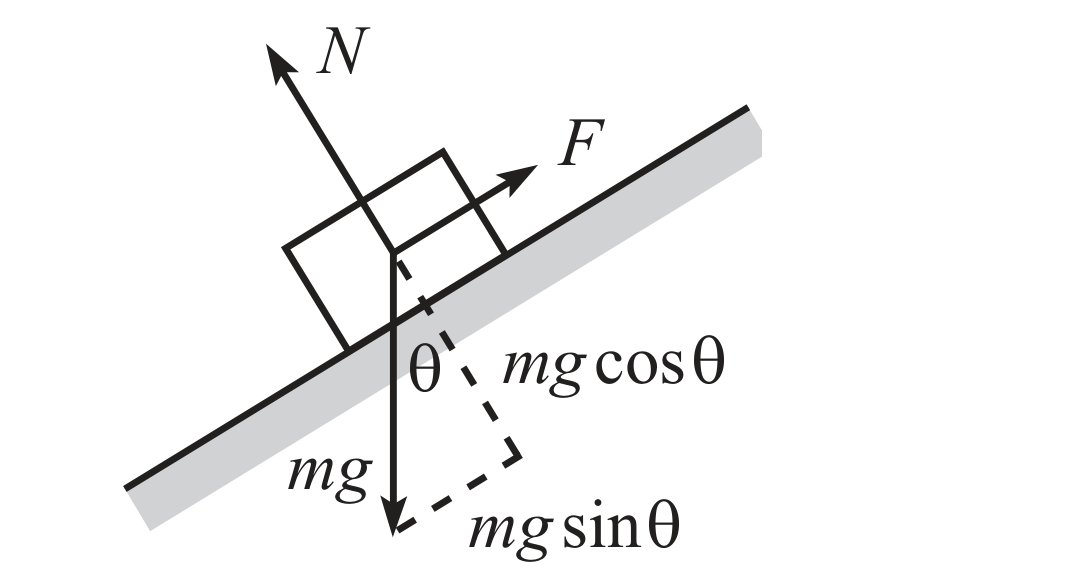
\includegraphics[width=\linewidth]{figures/sfig1.png}


These are equal, as they must be, because the net horizontal force on the block is zero. To maximize the value of $mg \sin\theta \cos\theta$, we can either take the derivative, or we can write it as $(mg/2) \sin 2\theta$, from which it is clear that the maximum occurs at $\theta = \pi/4$. The maximum value is $mg/2$.